\documentclass[12pt, a4paper, openright]{book}


\usepackage{amsmath}
\usepackage{graphicx}
\usepackage{hyperref}  % for citing URLs
\usepackage{listings}
\usepackage{float}
\usepackage{setspace}
\lstset{breaklines=true}
\pagestyle{plain}
\newcommand{\HRule}{\rule{\linewidth}{0.5mm}}

\topmargin       0in
\oddsidemargin   0in
\evensidemargin  0in
\headheight      0in
\headsep         0in
\topskip         0in
\textheight      9in
\textwidth       6.5in
%added on may 28 2014
\linespread{1.3}
%added on may 28 2014

\begin{document}

\frontmatter
\begin{titlepage}
\begin{center}
\begin{spacing}{1.0}

% Upper part of the page. The '~' is needed because \\
% only works if a paragraph has started.

% Title
%\HRule \\[0.4cm]
~\\[0.3cm]
{ \LARGE \bfseries Experimental implementation of a cognitive radio using OpenBTS, GNU Radio and spectrum sensing techniques\\[1.2cm] }

%\HRule \\[1.5cm]
\textbf{\large M. Tech. Dissertation}\\[1.2cm]

{Submitted in partial fulfilment of the requirements for the degree of\\[0.1cm]
Master of Technology\\[0.3cm]
by\\[0.3cm]}

{\LARGE Abrar Ahmad\\[0.1cm]}
{1100000\\[1.1cm]}
{Supervisor\\[0.1cm]}
{\LARGE Prof.~S~N~Merchant\\[1.3cm]}


\includegraphics[width=0.21\textheight]{iitbLogo}~\\[0.9cm]
Department of Electrical Engineering\\[0.2cm]
\textbf{\large IIT Bombay}\\[1.3cm]

%\textsc{\Large Master of Technology Project}\\[0.5cm]
%
%
%% Author and supervisor
%\begin{minipage}{0.4\textwidth}
%\begin{flushleft} \large
%\emph{Author:}\\
%Abrar \textsc{Ahmad}\end{flushleft}
%\end{minipage}
%\begin{minipage}{0.4\textwidth}
%\begin{flushright} \large
%\emph{Supervisor:} \\
%Prof.~S~N \textsc{Merchant}
%\end{flushright}
%\end{minipage}

\vfill

% Bottom of the page
{\large \today}

\end{spacing}
\end{center}
\end{titlepage}

\chapter*{\centering{Abstract}}
Wireless networks are currently regulated by fixed spectrum assignment policy
which results in inefficient utilization of the spectrum. In the last few
years there has been a drastic increase in the mobile services, which in turn
has increased the demand for limited radio spectrum. Hence there is a need to
change the conventional static spectrum assignment policy and make efficient
utilization of spectrum. Cognitive Radio (CR) emerged as a new paradigm to
address the spectrum underutilization problem.  CR enables opportunistic use
of the radio-frequency spectrum by allowing Secondary/Un-licensed users to
utilize licensed bands under the condition that they should not cause the
interference with the Primary/Licensed users. Secondary users utilize the
detected free bands and leave them when the corresponding primary radio
emerges.

A USRP based two frequency CR Test-Bed and a four frequency CR Test-Bed has been
developed using GNURadio and OpenBTS to demonstrate these properties of
cognitive radio. Primary and secondary users are made to coexist with no
effect on the primary radio. Energy detection spectrum sensing technique is
used to detect the free bands also known as the spectrum holes. We demonstrate
that secondary users utilize these spectrum holes and vacate them whenever
primary users want to use them.


\setcounter{tocdepth}{2}
\tableofcontents

\listoffigures
\setlength{\parindent}{0em}
\setlength{\parskip}{1em}
\setlength\arraycolsep{2pt}

\mainmatter
\chapter{Introduction}
\pagenumbering{arabic}
\thispagestyle{empty}
\section{Motivation}
Due to the rapid increase of mobile phones and other wireless communication 
devices, 
there is a need for efficient utilization of the available radio spectrum.
The Spectrum Policy Task Force, a group under the Federal Communications  
Commission (FCC) in the United States, published a report in 2002 saying 
\cite{repFCC}: 
\begin{quote}
``In many bands, spectrum access is a more significant problem than physical
scarcity of spectrum, in large part due to legacy command-and-control 
regulation that limits the ability of potential spectrum users to obtain such 
access.''
\end{quote}
If we scan the spectrum in metropolitan cities which are heavily used regions,
we find that some frequency bands are unoccupied most of the time\cite{staple04}. These 
are referred to as spectrum holes. A spectrum hole is a band of frequencies 
assigned to a primary user, but, at a particular time and specific geographic 
location, the band is not being utilized by that user\cite{kolodzy01}.

\begin{figure}
\centering
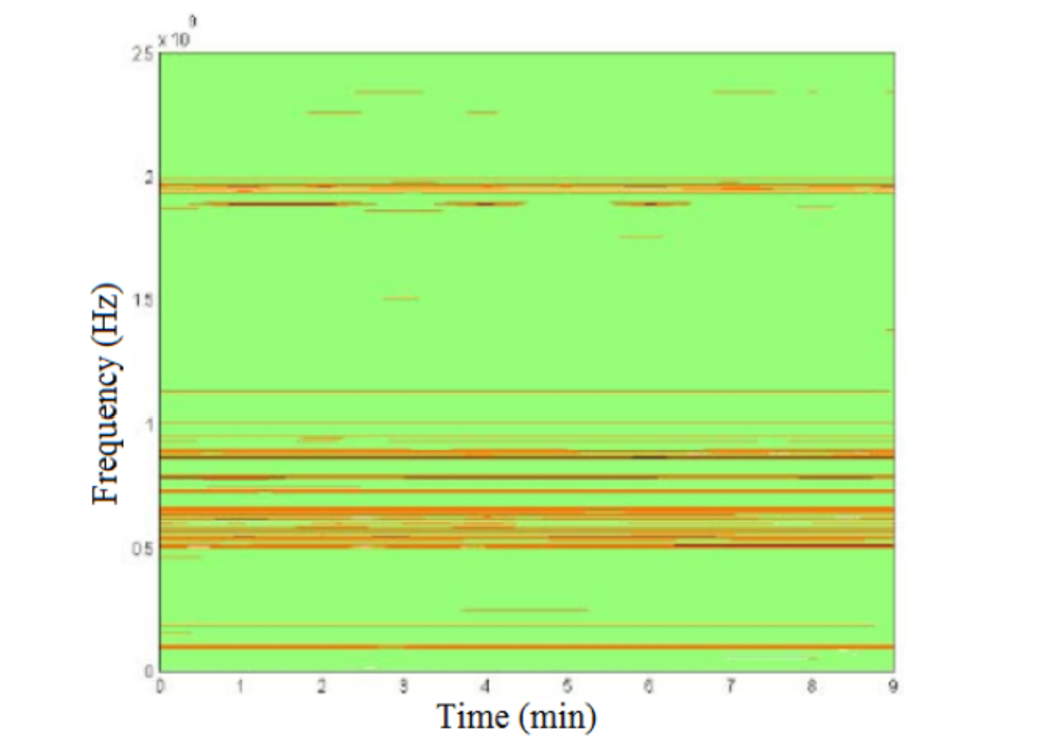
\includegraphics[width=0.7\textwidth]{../images/freqUsage}
\caption[Frequency usage of Spectrum Band]{Frequency usage of Spectrum Band {\cite{kranthi13}}}
\label{frequencyUsage}
\end{figure}


This problem of inefficient utilization of spectrum can be solved by allowing 
secondary users which are non licensed, to access these spectrum holes.
Cognitive radio which includes software defined radio, is a means to 
accomplish this by utilizing these spectrum holes intelligently and 
efficiently\cite{haykin05}\cite{mitola99}\cite{mitola00}. It uses one of the spectrum sensing techniques to 
identify the spectrum holes in the radio spectrum.


\section{Cognitive Radio}
A cognitive radio is an intelligent radio whose primary objective is efficient
utilization of the radio spectrum. It can be programmed and configured 
dynamically. It works on the principle of understanding-by-building to learn 
from the surrounding environment and adapt to changes in the RF stimuli by 
making corresponding changes in operating parameters. The transceiver is 
designed to find an unoccupied channel in the vicinity and utilize it for 
transmission. It enables coexistence of primary licensed users and secondary 
unlicensed users. Whenever a primary user wants to occupy the channel which is
currently in use by secondary users, it finds some other unoccupied channel in
the vicinity and secondary users migrate seamlessly to this new channel thus 
vacating the previously used channel for primary users.  

\section{Contribution of this Thesis}
An experimental setup is developed which demonstrates the presence of 
secondary users along with primary users in the existing GSM network and 
utilizing the already existing resources there by increasing the total 
mobiles in the network.
\begin{enumerate}
  \item A 2-frequency band cognitive system is developed where secondary 
  users migrate to frequency $f2$ if frequency $f1$ is occupied an viceverca.
  \item A 2-frequency system is extended to a 4-frequency system where 
  we demonstrate that primary users are occupying two bands out of these four
  and secondary users occupy one out of the other two free bands.
  \item We have used energy detection spectrum sensing technique and CUSUM
  peak detection technique to detect the presence of primary users. Band 
  occupied by secondary users is continuously monitored to check if primary 
  users are trying to occupy that band and as soon as the request from primary
  users is detected a new free band is found out in the vicinity and utilized 
  by secondary users for transmission there by vacating the band for primary 
  users . 
\end{enumerate}

\section{Organization of this Thesis}
The rest of this document is organized as follows. Chapter 2 briefly describes the GSM 
architecture and its Um interface. Chapter 3 discusses about software defined radio, GNURadio 
software and Universal Software Radio Peripheral (USRP N210), the hardware used in this 
project.OpenBTS software is described in Chapter 4. 
SIM registration and calling using local network  is described in chapter 5.
Chapter 6 covers spectrum sensing techniques to detect the presence of primary users in the 
channel.  Chapter 7 and 8 covers implementation of 2-Frequency and
4-Frequency cognitive radio test-beds using GNU Radio
and OpenBTS. Experimental setup for our project, 
detailed description of what we have achieved in this 
project along with the flow chart of our work is also covered in these chapters.
The final chapter of this thesis 
is the conclusion of our project followed by future work. 

\chapter{Overview of traditional GSM networks}

\section{What is GSM?}
GSM, or Global System for Mobile Communications, is a European standard for
the Mobile telecommunications and it is considered as one of the most popular
standard worldwide.There are thirteen different frequency bands defined in GSM.
However, the 850 MHz, 900 MHz, 1800 MHz, and 1900 MHz bands are the most
commonly used. The frequency bands employed within each of the four ranges are
similarly organized. They differ essentially only in the frequencies, such that
various synergy effects can be taken advantage of; hence, here we give some
details only for the usage in the 900 MHz band.


In the 900 MHz band, a total of 70 MHz bandwidth is allocated, two 25-MHz
frequency bands for uplink and downlink and a 20 MHz unused guard band between
them. The MS transmits in the 890 to 915 MHz range (uplink) and the BTS
transmits in the 935 to 960 MHz (downlink) band. This corresponds to 124 duplex
channels, where each channel within a BTS is referred to as an Absolute Radio
Frequency Channel Number (ARFCN). This number describes a pair of frequencies,
one uplink and one downlink, and is given a channel index between C0 and C123,
with C0 designated as the beacon channel. An ARFCN could be used to calculate
the exact frequency (in MHz) of the radio channel. In the GSM 900 band, this is
computed by the following equations:

\begin{align}
F_{uplink}(n) &= 890 + 0.2*n \qquad & 1\leq{}n\leq{}124 \nonumber\\
F_{downlink}(n) &= F_{uplink}(n) + 45 \qquad & 1\leq{}n\leq{}124 \nonumber
\end{align}

Similar formulae are also defined for the other GSM frequency bands.


The principle component groups of a GSM network are as follows:
\begin{itemize}
\item The Mobile Station (MS)
\item The Base Station System (BSS)
\item The Network Switching System(NSS)
\end{itemize}


\begin{figure}[h]
\centering
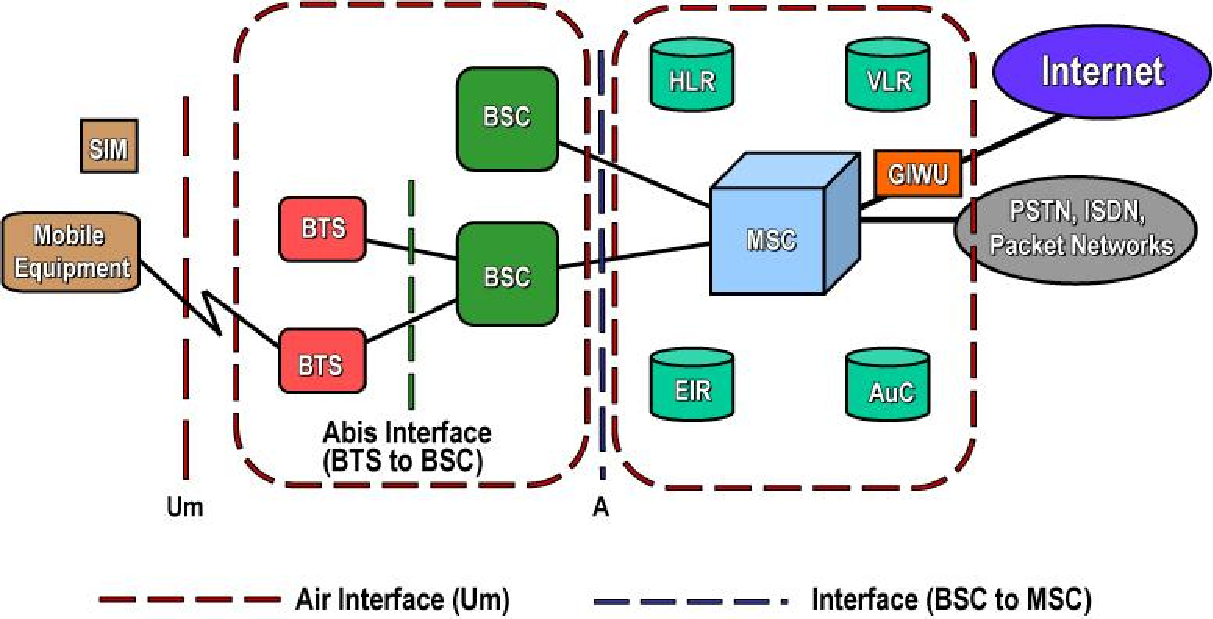
\includegraphics[width=1\textwidth]{gsmArch}
\caption[The conventional GSM architecture]{The conventional GSM architecture.
\emph{Source:
\url{http://www.hill2dot0.com/wiki/index.php?title=Image:G2407\_{}GSM-Architecture.jpg} 
[Accessed on Oct 22, 2013]}}
\label{gsmArch}
\end{figure}

\subsection{Mobile Station}
The MS consists of two parts, the Mobile Equipment (ME) and Subscriber
Identity module (SIM). The ME has an identity number called the International
 Mobile Equipment Identity (IMEI) associated with it, which is unique for
that particular device and permanently stored in it.The SIM card consists
the International Mobile Subscriber Identity(IMSI) number which is used
to identify the subscriber to the system. The IMEI and the IMSI are independent
of each other and hence allow personal mobility.

\subsection{Base Station System}
The GSM Base Station System is the equipment located at a cell site. It
comprises of a combination of digital and RF equipment. The BSS provides
the link between the MS and the Mobile Services Switching Centre (MSC).
The BSS consists mainly of:
\begin{description}
\item[The Base Transceiver Station(BTS)]
The BTS contains the RF components that provide the air interface for
 a particular cell. This is the part of the GSM network which communicates
 with the MS. The antenna is included as part of the BTS.
\item[The Base Station Controller(BSC)]
The BSC provides the control for the BSS. The BSC communicates directly
with the MSC. The BSC may control single or multiple BTSs. Crucial functions
like radio channel link establishment, frequency hopping, and handovers from
one cell to another.

\end{description}

\subsection{Network Switching Subsystem}
The Network Switching Subsystem includes
the main switching functions of the GSM network. It also contains the databases
required for subscriber data and mobility management. Its main function is
to manage communications between the GSM network and other telecommunications
networks. The main components of the Network Switching System are:


\subsubsection*{Mobile Services Switching Centre(MSC)}
The MSC does call-switching
and its overall purpose is the same as that of any telephone exchange. When
the MSC provides the interface between the PSTN and the BSSs in the GSM
network it will be known as a Gateway MSC. In this position it will provide
the switching required for all MS originated or terminated traffic. Each
MSC provides service to MSs located within a defined geographic coverage
area. One MSC is capable of supporting a regional capital with approximately
 one million inhabitants.
The functions carried out by the MSC are: Call Processing, Operations and
Maintenance Support, Internetwork Interworking and Billing

\subsubsection*{Home Location Register (HLR)}
The HLR is a central database that contains the details of each mobile phone
subscriber that is authorized to use the GSM core network. The IMSI of
each SIM acts as a primary key to each HLR record. Each MSISDN is
also a primary key to the HLR record. The HLR data is stored
as long as a subscriber remains with the mobile phone operator.
Data stored in the HLR against each IMSI are, GSM services that the
subscriber has requested, GPRS settings to allow the subscriber to
access packet services, current location of the subscriber, etc.

\subsubsection*{Visitor Location Register (VLR)}
The VLR is a database of the subscribers who have roamed into the jurisdiction
of the MSC which it serves. Each main base station in the network is served by
exactly one VLR, hence a subscriber cannot be present in more than
one VLR at a time.The data stored in the VLR has either been received
from the HLR, or collected from the MS. Data stored includes: IMSI
(the subscriber's identity number), authentication data, MSISDN,
GSM services that the subscriber is allowed to access, the HLR address
of the subscriber.



\section{Um Interface}
The Um interface is the air interface of the GSM mobile telephone standard.
It is the interface between the MS and the BTS. It is called Um because it
is the mobile analog to the U interface of ISDN. Um is defined in the
GSM 04.xx and 05.xx series of specifications.


The layers of GSM are initially defined in GSM 04.01 Section 7 and roughly
follow the OSI model. Um is defined in the lower three layers of the model.

\subsection{Physical Layer (L1)}
The Um physical layer is defined in the GSM 05.xx series of specifications,
 with the introduction and overview in GSM 05.01. For most channels,
Um L1 transmits and receives 184-bit control frames or 260-bit vocoder
frames over the radio interface in 148-bit bursts with one burst per
timeslot. There are three sublayers:

\subsubsection*{Radiomodem}
 
This is the actual radio transceiver. GSM uses 8PSK modulation with 1 bit per
symbol which produces a 13/48 MHz (270.833 kHz or 270.833 K symbols/second)
symbol rate and a channel spacing of 200 kHz. Since adjacent channels overlap,
the standard does not allow adjacent channels to be used in the same cell. The
standard defines several bands ranging from 400 MHz to 1990 MHz.GSM is frequency
 duplexed, meaning that the network and MS transmit on different frequencies,
allowing the BTS to transmit and receive at the same time. Transmission from
the network to the MS is called the ``downlink" and that from the MS to the network
is called the ``uplink". The GSM uplink and downlink bands are separated by 45 or
50 MHz. Uplink/downlink channel pairs are identified by an index called the
ARFCN. Within the BTS, these ARFCNs are given arbitrary carrier indexes
C0..Cn-1, with C0 designated as a Beacon Channel and always operated at constant
 power. The radio channel is time-multiplexed into 8 timeslots, each with a
duration of 156.25 symbol periods. These 8 timeslots form a frame of 1,250
symbol periods. The capacity associated with a single timeslot on a single
ARFCN is called a physical channel (PCH) and referred to as ``CnTm" where n is
a carrier index and m is a timeslot index (0-7).Each timeslot is occupied by
a radio burst with a guard interval, two payload fields, tail bits, and a
midamble.


\subsubsection*{Multiplexing and Timing}
GSM uses TDMA to subdivide each
radio channel into as many as 16 traffic channels or as many as 64 control
channels. The multiplexing patterns are defined in GSM 05.02.Each physical
channel is time-multiplexed into multiple logical channels according to
the rules of GSM 05.02. Traffic channel multiplexing follows a 26-frame
(0.12 second) cycle called a "multiframe". Control channels follow a
51-frame multiframe cycle. The C0T0 physical channel carries the
synchronization channel(SCH), which encodes the timing state of the
BTS to facilitate synchronization to the TDMA pattern.


\subsubsection*{FEC Coding} The coding sublayer provides forward error
correction. As a general rule, each GSM channel uses a block parity code
(usually a Fire code), a rate-1/2, 4th-order convolutional code and a
4-burst or 8-burst interleaver.



\subsection{Data Link Layer(L2)}
The Um data link layer, LAPDm, is defined in GSM 04.05 and 04.06.
LAPDm is the mobile analog to ISDN's LAPD.

\subsection{Network layer(L3)}
The Um network layer is defined in GSM 04.07 and 04.08 and has three sublayers.
A subscriber terminal must establish a connection in each sublayer before
accessing the next higher sublayer.

\begin{description}
\item[Radio Resource (RR)] This sublayer manages the assignment and
release of logical channels on the radio.

\item[Mobility Management (MM)] This sublayer authenticates users and
tracks their movements from cell to cell. It is normally terminated in
the VLR or HLR.

\item[Call Control (CC)] This sublayer connects telephone calls and is
taken directly from ITU-T Q.931. GSM 04.08 Annex E provides a table of
corresponding paragraphs in GSM 04.08 and ITU-T Q.931 along with a summary
of differences between the two. The CC sublayer is terminated in the MSC.

\end{description}

The access order is RR, MM, CC. The release order is the reverse of that.
Note that none of these sublayers terminate in the BTS itself. The standard
GSM BTS operates only in layers 1 and 2.
\chapter{OpenBTS}

\section{What is OpenBTS?}
OpenBTS is a Unix application that uses a software radio to present a GSM Um interface to handsets and uses a SIP softswitch or PBX to connect calls.(You might even say that OpenBTS is a simplified form of IMS that works with 2G feature-phone handsets). The combination of the global -standard GSM air interface with low cost VoIP backhaul forms the basis of a new type of cellular network that can be deployed and operated at substantially lower cost than existing technologies in many applications, especially rural cellular deployments and private cellular networks in remote areas.

\section{The OpenBTS Application Suite}
A complete OpenBTS P2.8 installation comprises several distinct applications:

\begin{description}
\item[OpenBTS] The actual OpenBTS application, containing most of the GSM stack above the radio modem.
\item[Transceiver] The software radio modem and hardware control interface.
\item[Asterisk] The VoIP PBX in the standard public release configuration.
\item[Smqueue] The store-and-forward server for text messaging.
\item[Subscriber Registry] A database of subscriber information that replaces both the Asterisk SIP registry and the GSM Home Location Register (HLR).
\item[Other Servers] Other optional GSM services, beyond speech and text messaging, are supported through external servers.
\end{description}

The OpenBTS and Transceiver applications must run inside each GSM/SIP access point. The Asterisk and the subscriber registry applications are communicated through the filesystem and therefore must run on the same computer, but that computer can be remote from the access point. smqueue and the other servers can run anywhere and may have multiple instances.

 \subsection{OpenBTS}
The OpenBTS application contains:
\begin{itemize}
\item L1 Time division multiplexing(TDM) functions (GSM 05.02)
\item L1 Forward error correction(FEC) functions (GSM 05.03)
\item L1 closed loop power and timing controls (GSM 05.08 and 05.10)
\item L2 Link access protocol on Dm-channel (LAPDm) (GSM 04.06)
\item L3 radio resource management functions (GSM 04.08)
\item L3 GSM-SIP gateway for mobility management
\item L3 GSM-SIP gateway for call control
\item L4 GSM-SIP gateway for text messaging
\end{itemize}

The general design approach of OpenBTS is avoid implementing any function above L3, so at L3 or L4 every subprotocol of GSM is either terminated locally or translated through a gateway to some other protocol for handling by an external application. Similarly, OpenBTS itself does not contain any speech transcoding functions above the L1 FEC parts.

\subsection{Transceiver}
The transceiver application performs the radio modem functions of GSM 05.05 and manages the Gigabit Ethernet interface
(USB2 interface, in case
of USRP1 or older models) to the radio hardware.

\subsection{Asterisk}
OpenBTS uses a SIP switch or PBX to perform the call control functions that would normally be performed by the mobile switching center in a conventional GSM network, although in most network configurations this switching function is distributed over multiple switches. These switches also provide transcoding services. In OpenBTS P2.8 the standard SIP switch is Asterisk 1.8.

\subsection{Subscriber Registry}
OpenBTS uses a modified SIP registry as a substitute for the home location register found in a conventional GSM network. OpenBTS also relies on Asterisk for any transcoding functions.

\subsection{Smqueue}
Smqueue is a store-and-forward server that is used for text messaging in the OpenBTS system. Smqueue is required to send a text message from one MS to another, or to provide reliable delivery of text messages to an MS from any source.

\subsection{Network Organization}
In the simplest network, with a single access point, all of the applications
in the suite run inside the access point on the same embedded computer. Figure
\ref{btsSimple} describes this.



\begin{figure}
\centering
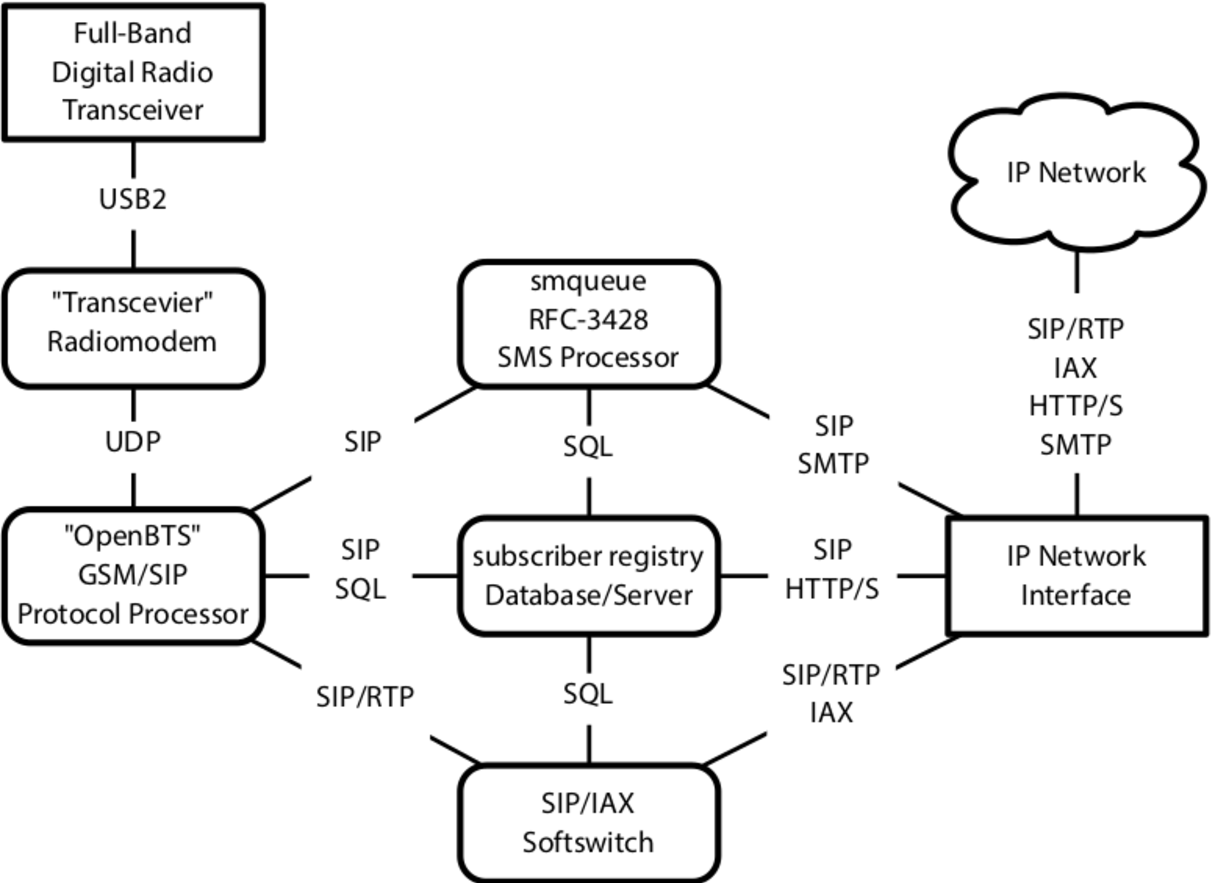
\includegraphics[width=1\textwidth]{../images/btsSimple}
\caption[Network Organization of OpenBTS]{Network Organization of OpenBTS {\cite{openbtsMan}}.}
\label{btsSimple}
\end{figure}

The smqueue block handles SMSs.
The subscriber registry database contains the details of all registered users and it
maps the registered IMSIs to corresponding dialling numbers. The softswitch connects
speech calls (e.g. Asterisk, FreeSwitch). The transceiver performs radio modem
functions and manages the Gigabit Ethernet interface (USB2 interface, in case
of USRP1 or older models) to the USRP device. The OpenBTS itself is the GSM
implementation from the TDMA part of L1 up through L3 and the L3/L4 boundary.
It has a SIP interface to communicate with the other blocks like smqueue, subscriber
registry, etc.


In larger network, with more than one access points, one of the BTS can behave as a master
and provide servers to the rest of them. Figure \ref{fig:btsLarge} describes a network with two access points
where a master access points is providing servers to the other one.
The Transceiver applications and the OpenBTS must run in each GSM/SIP access point.
The Asterisk and the Subscriber Registry applications (SIPAuthServe) communicate via the
filesystem and hence must run in the same computer, but that computer can be remote to the
access point. SMQueue and other servers can run in any access point and can have multiple
instances.
\begin{figure}
  \centering
    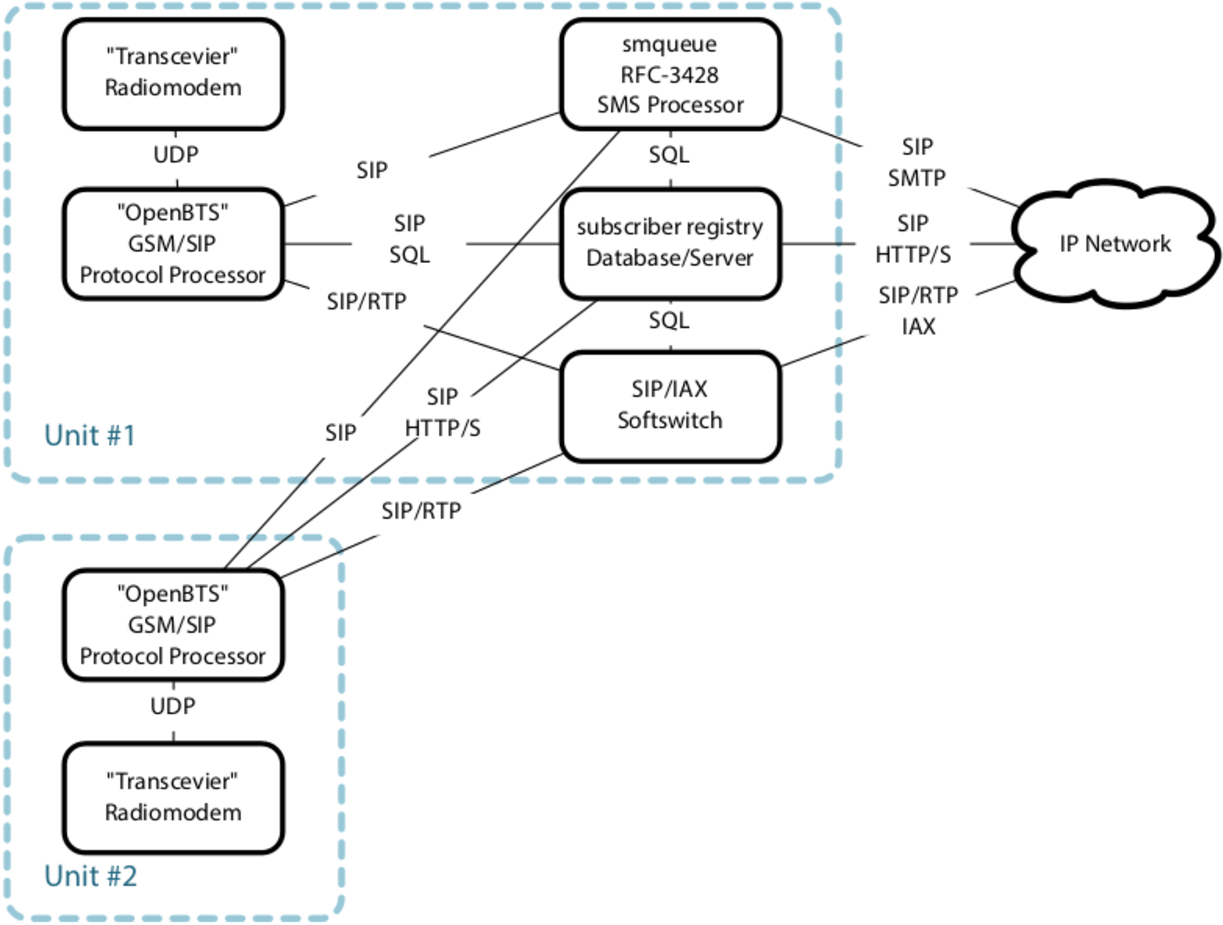
\includegraphics[width=\textwidth]{../images/btsLarge}
  \caption[OpenBTS network with two access points]{Two access points with unit 
  \#1 providing servers for both {\cite{openbtsMan}}.}
  \label{fig:btsLarge}
\end{figure}







\chapter{Spectrum Sensing}

Due to limited availability of spectrum resource, there is a serious impact on 
the emerging mobile applications. Hence there is a need to efficiently utilize
the available radio spectrum. The problem right now is not the physical scarcity
of the radio spectrum rather the inefficient use of the spectrum. Solution to 
this is cognitive radio. The major problems in cognitive radio is detection of 
primary users in the licensed spectrum and enable secondary users to quit the 
frequency band as quickly as possible if the corresponding primary radio emerges
to avoid interference to primary users. This technique is called spectrum 
sensing. Spectrum sensing is the first step to implement cognitive radio system.

There are various methods for local spectrum sensing proposed by researchers.

The following section describes three important methods:
\begin{enumerate}
	\item Energy detection
	\item matched filter detection 
	\item cyclo stationarity detection
\end{enumerate}

\section{Energy Detection}

Measuring the energy of a particular band is one of the simplest techniques to 
detect the presence of primary users in that band. It is one of the most widely
used technique to detect spectrum holes as it requires no a priori knowledge of 
the primary radio. Apart from this major advantage the technique is very cost 
efficient and less complex compared to other techniques. 
We calculate the energy of the received radio spectrum and this energy is 
compared with a predefined energy detection threshold to conclude whether 
primary user is present or absent in the frequency of interest. This technique 
is an optimal one when we have absolutely no knowledge of the user occupying the
channel in advance. The following block diagram describes energy detection 
technique:

Block diagram for energy detection technique from stage one report here:


As described in the energy detection block diagram, it is basically a hypothesis
testing problem with two possible hypothesis $H0$ and $H1$. Hypothesis $H1$ concludes 
the presence of primary users in the band of interest and hypothesis $H0$ 
concludes their absence. And energy detection technique is basically about 
distinguishing between these two hypothesizes.[3 from stage one report]

\begin{align}
x(t) & = n(t); & H0 \nonumber \\
x(t) & = hs(t)+n(t); & H1 \nonumber
\end{align}

where $x(t)$ is signal received by secondary user and $s(t)$ is primary radio 
signal, $n(t)$ is additive white Gaussian noise (AWGN) and $h$ is the amplitude gain
of the channel. $s(t)$ and $n(t)$ are assumed to be independent of each other. 
Signal detection is performed using an energy detector and compute decision 
statistics $Y$ which corresponds to energy collected in observation time $Y$ and 
bandwidth $W$ and comparing this statistics to a predetermined threshold. Energy 
detection is implemented using average periodogram analysis which is covered in 
later part of this report.


\section{Matched filter detection}
Matched filter is a linear filter used to match a particular transit waveform 
with the reference signal. The output is maximum when the match happens. When 
there is a priori knowledge of primary radio, matched filter technique is 
applied. Matched filter operation is equivalent to correlation operation in 
which the incoming signal is convolved with a filter whose impulse response is 
mirror and shifted version of reference signal. This output is then compared 
with the threshold for primary user detection. It is mathematically defined as:

\begin{equation*}
Y[n] = \sum_{k=-\infty}^{\infty}x[k]h[n-k]
\end{equation*}

$x$ is the unknown signal and $h$ is the impulse response of matched filter which is 
matched to reference signal for maximizing SNR. 

Block diagram of matched filter is given in fig:

There is a constraint on this technique. We need to have a prior information 
about the primary radio to perform matched filtering. However matched filter 
requires demodulation of primary signal which means it has information of 
primary radio both at the PHY layer and the MAC layer like operating frequency, 
modulation type, packet format bandwidth etc. But the cumbersome part is it has 
to achieve coherency with primary user by means of timing and carrier 
synchronization. This coherent detection is still achievable since primary 
signals have pilots, preambles etc to serve the purpose. 
The advantage of matched filter detection is when the information of the primary
user signal is known, it is optimal detection in stationary Gaussian noise. But 
the performance of matched filter detection depends on the accuracy of the 
information of primary radio. This technique also requires cognitive radio to 
have dedicated receiver for every type of primary user which in turn results in 
complex hardware and large power consumption. [4] kranti thesis

\section{Cyclostationarity detection}

This technique utilizes periodicity property of the received signal to detect 
presence of primary users. Periodicity property is generally exhibited by the 
communication signals due to sinusoidal carriers, pulse train, hopping sequences
etc. Due to this underlying periodicity most of the communication signals can be
modeled as cyclostationary processes[1from folder project on desktop]. This 
technique detects a random primary signal with a particular modulation type in a
background of noise and other modulated signals.

Cyclostationary feature detection is robust to noise and is a better performer 
than energy based detection in low SNR regions. This technique also requires a 
priori knowledge of the primary signal. Also this technique is computationally 
highly complex and the sensing time is also quiete long. Due the these reasons 
it is less commonly used than energy based detection.

Block diagram of cyclostationary detection is given in the figure:[14 from 
kranti thesis]


Diagram 

The detection is done by finding a unique cyclic frequency of the spectral 
correlation function of the received signal [4kranti]. The spectral correlation 
function is the Fourier transform of the cyclic autocorrelation function the 
spectral correlation function is defined as:
\begin{equation*}
        S(f,\alpha) = \int_{-\infty}^{\infty} R_{x}^{\alpha}(\tau)e^{-2 \pi f\tau}d\tau 
\end{equation*}

Where the cyclic autocorrelation function is defined by:
\begin{equation*}
    R_{x}^{\alpha} = E\{x(t+\tau)x^{*}(t-\tau)e^{-2 \pi \alpha t}\}
\end{equation*}

Here $x(t)$ is the signal received and $\alpha$ is the cyclic frequency. The spectral 
correlation function is also termed as cyclic spectrum.
This is a two dimensional transform unlike power spectral density which is 1 
dimensional. For successful detection under cyclo-stationary based spectrum 
sensing, we need a priori knowledge of the cyclo-stationary features of the 
received signal only. However matched filtering is the optimal solution when we 
completely know about received signal in advance.
This technique doesn't work well when the underlying noise is stationary. More 
over channel fading destroys the property of cyclo stationarty of the received 
signal and is also susceptible to sampling clock offset. 


Comparision of various spectrum detection techniques

Diagram from kranti's thesis 









The figure compares various spectrum sensing techniques on the basis of their 
accuracy and complexity. We can see that energy detection technique is the least
accurate and least complex of all where as matched filtering is most complex and
highly accurate. Other techniques lie in between with some having more accuracy 
and some less complex. There is no ideal detector that suits all occasions. Thus
decisions, compromises and tradeoffs must be made depending on primary radio 
type, transmission and propagation characteristics, characteristics of secondary
user receiver, and etc [2 from karanti thesis].

\section{Implementaton of energy detection technique}
We have used energy detection technique for spectrum sensing in our project for 
the detection of primary users in the band of interest. Average periodigram 
analysis is a method to implement energy detection technique of spectrum 
sensing. This section describes average periodogram analysis.  Implementation of
wide band spectrum analyzer using this technique is also described in this 
section.

\subsection{Average periodogram anaylsis}
Average Periodogram analysis estimates the power spectrum of the received signal
and it is based on the Discrete Fourier Transform (DFT) of finite length 
segments of signal. In this technique signal is sectioned into finite length 
segments and periodogram of each segment is calculated which are also referred 
to as modified periodograms. Then an average of all these modified periodogram 
is calculated.[8 from krantis report]

Let $X[n]; n = 0,1...L-1$ be the discrete time signal which is  divided into 
$M$ 
finite length segments of equal length, where $N$ is the length of each segment  
i.e. $ MN = L; X_{r}[n]; n = 0,1...N-1 $ is the $r$th segment and $ W[n]; n = 0,1...N-1 $ is 
the window applied to each segment. The modified periodogram for the $r$th segment
 is,
\begin{equation*}
    I_{r}[k] = \frac{1}{NU} \left| V_{r}[k]\right|^2     \qquad k = 0,1...N-1 
\end{equation*}
where $V_{r}[k]$ is a N point DFT and $U$ is normalization factor i.e. , 
$V_{r}[k] = DFT\{W[n]*X[n]\}$
and $U = \frac{1}{N}(\sum_{n-0}^{N-1} (W[n])^2)$
The PSD of $X[n]$ sequence is then the time averaged periodogram estimate ,
\begin{equation*}
    I[k] = \frac{1}{M}\left|\sum_{r=0}^{M-1}X_{r}[k]\right|
\end{equation*}

\section{Wide band spectrum analyzer}

GNU radio packages provide a tool for
wide band spectrum sensing 
called 
usrp\_spectrum\_sense.py. The program is provided in the appendix. 
It is used as
a basic code for wide band spectrum analyzer implementation. The output of this 
code is the magnitude squared of the FFT. This means for each FFT bin he output 
is $ Y[i] = re[X[i]]*re[X[i]] + im[X[i]]*im[X[i]]$. We can calculate the power by
taking square root of the output. We need $N$ time samples of $x(t)$ sampled at a 
sampling frequency of $F_{s}$ to use $N$ point complex FFT $X(\omega)$ analysis. An 
appropriate window function is to be selected to reduce spectral leakage and 
applied to these time samples. The output of the complex FFT will represent the 
frequency spectrum content as follows: The first value of the FFT output 
$(bin0 == X[0])$ is the passband centre frequency The first half of FFT spectrum 
($X[1]$ to $X[N/2-1]$) contains the positive baseband frequencies, which corresponds
to the passband spectrum from centre frequency to $+F_{s}/2$. The second half of the 
FFT ($X[N/2]$ to $X[N-1]$) contains the negative baseband frequencies, i.e. from 
$-F_{s}/2$ to centre frequency.


For our project purpose, we collected 1024 samples using a tuner centered at 
uplink frequency of our interest, say 900 MHz. 1024 is choosen as the number of 
FFT points because the number of FFT points has to be a power of 2 for the fast 
execution of the FFT algorithm. Default  sampling frequency is set as 10 MHz. 
The frequency resolution is therefore: 10 MHz / 1024 = 9.7656 MHz. The 
decimation is defined as dsp rate divided by sample rate. The UHD driver 
requires the decimation value to be an even number. The dsp rate is the actual 
hardware-level sampling rate of the USRP kit. It is the rate at which the USRP 
device takes analog samples from the external world and converts them to digital
form. The dsp rate of the USRP is 100 MHz. Hence we chose sampling frequency to 
be 10 MHz which gives a decimation value of: 100 MHz / 10 MHz = 10.

\chapter{Implementation of cognitive radio using OpenBTS}

In our project we are able to successfully demonstrate the
coexistence of primary users and secondary users in the same 
frequency channel in the
GSM band. In order to accomplish this, we have implemented
a cognitive radio which detects the spectrum holes in the
radio spectrum and enables secondary users to utilize these 
for communication. An experimental setup has been  
developed for this demonstration using OpenBTS and GNU 
radio software and USRP N210 as hardware.

Experimental setup diagram:


\section{Description of setup}
The figure above describes the experimental setup for a
two-frequency system. The primary system has only
one USRP as an RF front and it runs OpenBTS. The 
secondary system has two USRP kits connected to it and one of them
runs OpenBTS and the other GNURadio.
This secondary system has cognitive capabilities. 
To provide cognitive capabilities it was required that 
OpenBTS and GNU radio run together in the same system and 
talk to each other which was challenging. Secondary system
continuously senses the frequency band of interest and does 
decision making depending upon the analysis of the data 
collected and changes its parameters accordingly so that 
primary and secondary users coexist. The spectrum sensing 
is accomplished by using GNU radio. Also we made GNU radio 
and OpenBTS coordinate to behave in appropriate manner and 
take dynamic decisions as and when required to make over all
system behave in a cognitive manner.

First a two-frequency cognitive system is developed.
For this two GSM bands are used with centre frequency
945 MHz (F1) and 950 MHz (F2). Secondary users are made to occupy
one of these two bands say F1. Then we make the primary users 
enter the same band. This results in an increase in energy 
levels in this band which is sensed by the secondary system 
as it continuously scans this band. Immediately
secondary users are shifted to other frequency band (F2)
there by vacating F1 for primary users. Hence a two-frequency
cognitive system demonstrating coexistence of a pair of
primary and secondary users is accomplished. 

The whole technique is described using a flow graph below:

Flow graph here :

Now this two frequency system is expanded to a 
four frequency system where we have F1 = 936 MHz, 
F2 = 943 MHz, F3 = 950 MHz, F4 = 957 MHz. The experimental setup
is also expanded with two primary systems and one secondary
system. Each primary system has an USRP kit running OpenBTS and
the secondary system has two USRP kits connected to it, one for OpenBTS
and the other one for GNURadio, as we had previously in the two-frequency 
system.
 
Figure for 4 frequency system here:


Here we make a pair of primary users occupy one of the four
frequency channel say F2. We make secondary users use a frequency channel
say F1. Now the other pair of primary users try to enter frequency
F1 for communication. This is sensed by the secondary system 
and it tries to migrate secondary users to F2 which also happens to be 
occupied already. Our secondary system detects that F2 is occupied and
therefore moves on to find a spectrum hole in the four-frequency 
spectrum. It finds that frequency F3 is unoccupied and thus
allows secondary users to enter F3 and utilize it for communication.
The difference between a four-frequency system and a two-frequency system is 
that the secondary system in a four-frequency
system has to first check the presence of primary users before 
switching into a particular frequency channel.
This was not the case in the two-frequency system. In the
two-frequency system we assumed that the other band is always 
unoccupied at the time of switching as only a pair of primary
users existed and thereby only a single band is always unoccupied.


The following flow graph describes the four frequency cognitive system:

Flow graph here

The spectrum sensing is done by energy detection technique and
it was required that a proper threshold be set for decision making. 
A number of readings were taken to decide the noise level, energy 
level when only primary users were active and also energy levels 
when both primary users and secondary users were active in the same band 
for a short duration of time. The threshold value depends on the
power transmitted by the users and their distance from the USRP 
kit which is RF front for GNURadio. This distance dependency can 
be removed by setting the threshold quite lower than required so 
that even if the users move far away the decision making is not
affected. 






\section{CUSUM}
CUMSUM peak detection is also applied after energy detection to ensure that the
detected high energy in the band of interest is not due some  not relevant 
reason like random fluctuations in noise power etc but due to presence of 
primary radio in that band. This ensures high accuracy in primary radio 
detection and correct decision making.
CUSUM is basically a sequential analysis technique to monitor change detection. 
It is a criterion for deciding when to take corrective action. As the name 
implies CUSUM involves calculating cumulative sum. This makes it sequential. 
The samples from process  are assigned weights  and summed as followed,

\begin{align}
S_0 &= 0; \nonumber \\
S_{n+1} &= max(0, S_n + x_n - \omega_n) \nonumber
\end{align}
When the value of  exceeds a certain threshold value a change  in value has 
been found. This formula detects change only in positive direction. To detect 
change in negative direction we have to do min operation instead of max 
operation and the change in value is detected when goes below threshold.







\section{Tasks over the year}
The next section of this chapter gives a step by step description of tasks we 
accomplished during our project tenure. 

\begin{enumerate}

\item We began with exploring with what cognitive radio is and how it can be used 
in the already existing radio. We did literature survey on the ongoing work in 
context to cognitive radio. 
\item We learned GNU Radio software package starting from its installation. We 
also designed FM receiver using GNU Radio Companion to get use to the software. 
Also we tried and learn the codes of already existing signal processing blocks 
that GNU Radio provides.
\item GNU Radio applications are primarily written using the Python programming 
language and hence we learned Python language.
\item USRP N2 kit is used as hardware in our project. We got use to this kit and 
also did range testing of this kit to ensure distance is not a major factor in 
our decision making algorithm and can be neglected.
\item The next task was to understand the working of OpenBTS software. Starting 
from the installation of this software we registered our GSM SIM cards in the 
local network established by OpenBTS. We could perform calling and SMS sending 
between our phones using the local network established by Open BTS with USRP 
kit as hardware end.
\item Since spectrum sensing is major part of cognitive radio literature survey 
on various spectrum sensing techniques was done. We choose energy detection 
spectrum sensing technique for our project and so we did detail study of a 
technique called Average Periodogram Analysis to implement this method. We also 
simulated this technique in Matlab using various windowing methods and 
understand results. 
\item After all this we designed our problem statement and the flow graph of 
how we will approach the problem which we have included in the last chapter. 
Also we decided upon building the experimental setup which we have covered in 
the start of this chapter. 
\item  First key step to approach this problem was to run Open BTS and GNU 
Radio together in the same computer with two USRP kits connected one for Open 
BTS and other for GNU radio. It was a little tricky. \textbf{Why tricky u 
include here regarding the IP conflict an all}
\item The next was to build a two frequency cognitive system with a pair of 
primary and secondary users communicating in parallel and primary pair having 
higher priority when ever both try to use same radio band. Detail description 
of this is in the start of this chapter.
\item This two frequency system was expanded to four frequency system with two 
primary pair of users and one secondary pair of users coexisting. This 
demonstrated that both primary and secondary users can exist in the same GSM 
Network without affecting the existing system.
\end{enumerate}

\appendix
%\chapter{Codes}

\section{Code for the two-frequency system}


\subsection{freq2secondaryBTS.py}

This code was written to demonstrate the two-frequency system.
This code was written by modifying the already available program named 
``usrp\_spectrum\_sense.py'' that comes together with the GNURadio software
package. We set the 
default UHD device address to ``192.168.20.2'' because that is the IP address
of the USRP device we are using as a spectrum sensor. The default samping rate
was set to 1e6 i.e. 1MHz. The default FFT size is given as 'sampling rate /
channel bandwidth'. We wanted an FFT size of 1024 so we set the bandwidth to
976.56 Hz since 1 MHz / 976.56 Hz $\approx$ 1024.

The class 'my\_top\_block' was modified by replacing the lines:
\begin{lstlisting}[language=Python]

        self.channel_bandwidth = options.channel_bandwidth

        self.min_freq = eng_notation.str_to_num(args[0])
        self.max_freq = eng_notation.str_to_num(args[1])

        if self.min_freq > self.max_freq:
            # swap them
            self.min_freq, self.max_freq = self.max_freq, self.min_freq    
\end{lstlisting}
with the lines
\begin{lstlisting}[language=Python]
        self.channel_bandwidth = options.channel_bandwidth

        self.down_freq = eng_notation.str_to_num(args[0])
        self.up_freq = (self.down_freq) - 45e6    
\end{lstlisting}

The method 'set\_next\_freq' of the class 'my\_top\_block' was modified by
replacing
\begin{lstlisting}[language=Python]
        target_freq = self.next_freq
        self.next_freq = self.next_freq + self.freq_step
        if self.next_freq >= self.max_center_freq:
            self.next_freq = self.min_center_freq
\end{lstlisting}
with
\begin{lstlisting}[language=Python]
        target_freq = self.up_freq
\end{lstlisting}




In the code listing that follows we have listed only the functions that we
customized and the ones that we added.

\begin{lstlisting}[language=Python]
def main_loop(tb):
    startOpenBTS(tb.down_freq,tb)

    
def sub_loop(tb):

    # use a counter to make sure power is less than threshold
    # lowPowerCount = 0
    # lowPowerCountMax = 10
    print 'fft size', tb.fft_size
    N = tb.fft_size
    mid = N // 2
    cusum = 0
    counter = 0
    

    while 1:

        # Get the next message sent from the C++ code (blocking call).
        # It contains the center frequency and the mag squared of the fft
        m = parse_msg(tb.msgq.delete_head())

        # m.center_freq is the center frequency at the time of capture
        # m.data are the mag_squared of the fft output
        # m.raw_data is a string that contains the binary floats.
        # You could write this as binary to a file.



        center_freq = m.center_freq
        bins = 102
        power_data = 0
        noise_floor_db = 0 ## 10*math.log10(min(m.data)/tb.usrp_rate)
        
        for i in range(1, bins+1):
            power_data += m.data[mid-i] + m.data[mid+i]
        power_data += m.data[mid]
        power_data /= ((2*bins) + 1)
        
        power_db = 10*math.log10(power_data/tb.usrp_rate) - noise_floor_db
        power_threshold = -59.0
        
        

        #if (power_db > tb.squelch_threshold) and (power_db > power_threshold):
            #print datetime.now(), "center_freq", center_freq, "power_db", power_db, "in use"
            # lowPowerCount = 0
        #else:
        print datetime.now(), "center_freq", center_freq, "power_db", power_db
            # lowPowerCount += 1

        # if (lowPowerCount > lowPowerCountMax):
        # down_freq = center_freq + 45e6
        # startOpenBTS(down_freq)
        # break

        #cusum cusum cusum is here
        cusum = max(0, cusum + power_db - power_threshold)
        if (cusum > 0):
            counter += 1
            if (counter > 2):
                print "CUSUM is now positive!!!"
                down_freq = center_freq + 45e6
                quitOpenBTS(down_freq, tb)
                break

                
def startOpenBTS(downFrequency,tb):
    
    
    arfcn=int((downFrequency-935e6)/2e5)
    if (arfcn < 0):
        print "ARFCN must be > 0 !!!"
        sys.exit(1)
    print 'ARFCN=', arfcn
    #DB modifications
    t=(arfcn,)
    conn=sqlite3.connect("/etc/OpenBTS/OpenBTS.db")
    cursor=conn.cursor()
    cursor.execute("update config set valuestring=? where keystring='GSM.Radio.C0'",t)
    conn.commit()

    #start the OpenBTS
    f=subprocess.Popen(os.path.expanduser('~/ddpOpenBTS/runOpenBTS.sh'))
    f.wait()
    tb.msgq.delete_head()
    time.sleep(0.25)
    sub_loop(tb)


def quitOpenBTS(downFreq, tb):
    f=subprocess.Popen(os.path.expanduser('~/ddpOpenBTS/quitOpenBTS.sh'))
    f.wait()
    if downFreq <= 945e6:
        newDownFreq = downFreq + 10e6
    else:
        newDownFreq = downFreq - 10e6

    tb.up_freq = newDownFreq - 45e6
    print "new tb.up_freq: ", tb.up_freq
    startOpenBTS(newDownFreq, tb)
\end{lstlisting}






\section{Code for the four-frequency system}
\subsection{secondaryBTS.py}

Most of the code is similar to ``freq2secondaryBTS.py''. The only modified 
functions are listed below:

\begin{lstlisting}[language=Python]

def main_loop(tb):
    startOpenBTS(tb.down_freq,tb)


def sub_loop(tb):

    print 'fft size', tb.fft_size
    N = tb.fft_size
    mid = N // 2
    cusum = 0
    counter = 0
    

    while 1:

        # Get the next message sent from the C++ code (blocking call).
        # It contains the center frequency and the mag squared of the fft
        m = parse_msg(tb.msgq.delete_head())

        # m.center_freq is the center frequency at the time of capture
        # m.data are the mag_squared of the fft output
        # m.raw_data is a string that contains the binary floats.
        # You could write this as binary to a file.



        center_freq = m.center_freq
        bins = 102
        power_data = 0
        noise_floor_db = 0      ##  10*math.log10(min(m.data)/tb.usrp_rate)
        
        for i in range(1, bins+1):
            power_data += m.data[mid-i] + m.data[mid+i]
        power_data += m.data[mid]
        power_data /= ((2*bins) + 1)
        
        power_db = 10*math.log10(power_data/tb.usrp_rate) - noise_floor_db
        power_threshold = -70.0
        
        print datetime.now(), "center_freq", center_freq, "power_db", power_db

        #cusum cusum cusum is here
        cusum = max(0, cusum + power_db - power_threshold)
        if (cusum > 0):
            counter += 1
            if (counter > 2):
                print "CUSUM is now positive!!!"
                down_freq = center_freq + 45e6
                quitOpenBTS(down_freq, tb)
                break
        else:
            counter = 0




def startOpenBTS(downFrequency,tb):
    arfcn=int((downFrequency-935e6)/2e5)
    if (arfcn < 0):
        print "ARFCN must be > 0 !!!"
        sys.exit(1)
    print 'ARFCN=', arfcn
    #DB modifications
    t=(arfcn,)
    conn=sqlite3.connect("/etc/OpenBTS/OpenBTS.db")
    cursor=conn.cursor()
    cursor.execute("update config set valuestring=? where keystring='GSM.Radio.C0'",t)
    conn.commit()

    #start the OpenBTS
    f=subprocess.Popen(os.path.expanduser('~/ddpOpenBTS/runOpenBTS.sh'))
    f.wait()
    tb.msgq.delete_head()
    time.sleep(0.25)
    sub_loop(tb)
              

def quitOpenBTS(downFreq, tb):
    f=subprocess.Popen(os.path.expanduser('~/ddpOpenBTS/quitOpenBTS.sh'))
    f.wait()    
    newDownFreq = getNewChannel(downFreq, tb)
    startOpenBTS(newDownFreq, tb)

        

def getNewChannel(downFreq, tb):
    newDownFreq = downFreq + 7e6
    if newDownFreq > 960e6:
        newDownFreq = 936e6

    tb.up_freq = newDownFreq - 45e6
    print "new tb.up_freq: ", tb.up_freq
    tb.msgq.delete_head()
    time.sleep(0.25)

    print 'fft size', tb.fft_size
    N = tb.fft_size
    mid = N // 2
    cusum = 0
    counter = 0
    loopcounter = 0
    

    while loopcounter < 10:

        # Get the next message sent from the C++ code (blocking call).
        # It contains the center frequency and the mag squared of the fft
        m = parse_msg(tb.msgq.delete_head())


        center_freq = m.center_freq
        bins = 102
        power_data = 0

        
        for i in range(1, bins+1):
            power_data += m.data[mid-i] + m.data[mid+i]
        power_data += m.data[mid]
        power_data /= ((2*bins) + 1)
        
        power_db = 10*math.log10(power_data/tb.usrp_rate)
        power_threshold = -70.0
        
        
        print datetime.now(), "center_freq", center_freq, "power_db", power_db
        print "precheck"

        #cusum cusum cusum is here
        cusum = max(0, cusum + power_db - power_threshold)
        loopcounter += 1
        if (cusum > 0):
            counter += 1
            if (counter > 2):
                print "CUSUM is now positive!!!"
                newDownFreq = getNewChannel(newDownFreq, tb)
                break
        else:
            counter = 0
    return newDownFreq

\end{lstlisting}




\section{primaryBTS.py}
\begin{lstlisting}[language=Python]
#!/usr/bin/env python


import sys
import sqlite3
import os
import re

def main_loop():
    usage = "usage: %prog channel_freq"
    if len(sys.argv) != 2:
        print 'usage:', sys.argv[0], 'channel_freq'
        sys.exit(1)


    center_freq = int(re.match(r'\d+', sys.argv[1]).group())*1e6
    startOpenBTS(center_freq)

def startOpenBTS(frequency):            
    
    arfcn=int((frequency-935e6)/2e5)
    print 'ARFCN=', arfcn
    
    #DB modifications
    t=(arfcn,)
    conn=sqlite3.connect("/etc/OpenBTS/OpenBTS.db")
    cursor=conn.cursor()
    cursor.execute("update config set valuestring=? where keystring='GSM.Radio.C0'",t)
    conn.commit()
    
    #start the OpenBTS
    f=os.popen('~/ddpOpenBTS/runOpenBTS.sh')
    f.close()
              

if __name__ == '__main__':

    try:
        main_loop()

    except KeyboardInterrupt:
        pass

\end{lstlisting}


\section{runOpenBTS.sh}
\begin{lstlisting}[language=bash]
#!/bin/bash

sudo echo "Hi, this script starts OpenBTS in Ubuntu 12.04!"
sudo service asterisk restart
sudo gnome-terminal -x sh -c "sudo asterisk -r" &

#cd ~/OpenBTS/
#sudo gnome-terminal --tab -e "sudo smqueue/trunk/smqueue/smqueue" \
#   --tab -e "sudo subscriberRegistry/trunk/sipauthserve" &

cd ~/OpenBTS/openbts/trunk/apps/
sudo gnome-terminal --tab -e "sudo ../../../smqueue/trunk/smqueue/smqueue" \
    --tab -e "sudo ../../../subscriberRegistry/trunk/sipauthserve" &

#sudo gnome-terminal -x sh -c "sudo ./OpenBTS" &
#sudo gnome-terminal -x sh -c "sudo ./OpenBTSCLI" &
sudo gnome-terminal --tab -e "sudo ./OpenBTS" \
    --tab -e "sudo ./OpenBTSCLI" &
cd ~

\end{lstlisting}


\section{quitOpenBTS.sh}
\begin{lstlisting}[language=bash]
#!/bin/bash

sudo echo "Hi, this script turns OpenBTS off in Ubuntu 12.04!"

sudo killall transceiver smqueue sipauthserve OpenBTSCLI asterisk
\end{lstlisting}








\backmatter
\bibliographystyle{plain}
\bibliography{thesis2}

\end{document}
